\section{Background}
\subsection{Unmanned Aerial Systems}
Any aircraft flying without a pilot on board is referred to in the Convention on International Civil Aviation (Doc 7300), signed at Chicago on 7 December 1944 and amended by the ICAO Assembly as a “pilot-less aircraft.” Today we call these aircraft “unmanned” rather than “pilotless.” Unmanned aircraft (UA) includes a broad spectrum from meteorological balloons that fly freely to highly complex aircraft piloted from remote locations by licensed aviation professionals. The latter is part of the category referred to as “remotely piloted aircraft” or RPA that operate as part of a system, a remotely piloted aircraft system (RPAS).

RPAS are creating a new industry with large economic potential. They offer a vast range of capabilities and sophistication. Their associated technologies, designs, and operating concepts are evolving rapidly. It is within this context that States are being challenged with the safe and efficient integration of RPAS into environments shared by a highly regulated and well-established manned aircraft industry. According to size\cite{ICAO}
\subsection{UAS description}
Unmanned Aircraft Systems (UAS). An aircraft that does not carry a human operator and is capable of flight under remote control or autonomous programming. AUA is designed to be recoverable but can be expendable and can carry a lethal or non-lethal payload. UA is rotary or fixed-wing aircraft or lighter-than-air vehicles, capable of flight without an onboard crew. The UA includes the aircraft and integrated equipment (propulsion, avionics, fuel, navigation, and communication systems)\cite{Joint}
\subsection{UAS components} 
\begin{itemize}

\item Payload:  UAS payloads include sensors, communications relay, weapons, and cargo. Payloads may be internally or externally carried 
\item Sensors: Most today’s payloads are imaging sensors, such as electro-optical (EO), infrared (IR), and radar (synthetic aperture radar [SAR], inverse synthetic aperture radar [ISAR], and maritime search radar). Also, there are ground, surface and maritime moving target indicators, light detection and ranging (LIDAR), automated identification system (AIS), measurement and signature intelligence, and signals intelligence (SIGINT) sensors. 
\item Communications Relay: Communications relay payloads provide the capability to extend voice and data transmissions via the UAS. 
\item Control elements: the control element, whether ground-based, sea-based, or airborne, handles multiple mission aspects, such as Command and Control (C2), mission planning, payload control, and communication 
\item Data Link: Data links include all means of communicating among the UA, UAS control element, and user, and are used for any means of data transfer. \cite{Joint}
\end{itemize}

\subsection{UAS classification}
\subsubsection{Motor Propulsion type}
\begin{itemize}
\item Fixed-wing UAS: Fixed wing UAS are characterized to have a straightforward structure, aerodynamically efficient, that allows to reach high speeds and have a higher efficiency than multirotor platforms, due to the lower power consumption. The landing and take-off procedure present a difficulty to these types of UAS due to the necessity of a runway.
\item Rotatory wing: They are composed of 2 or more rotor. Its main characteristics are the ability to perform vertical take-off and landings, in addition to having a great maneuverability and flight precision. Its main disadvantage is due to its more complex electronics structure, sacrifice flight autonomy.\cite{Luis_Fernadno}
\end{itemize}
\begin{figure}[H]
\centering
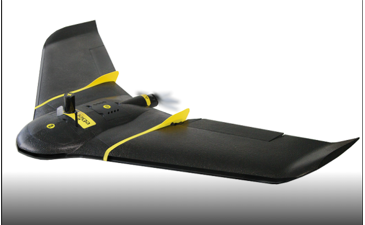
\includegraphics[width=10cm,height=10cm,keepaspectratio]{imagenes/eBee.PNG}
\caption{Fixed-wing UAS platform}
\label{fig:fixed-wing_UAS}
\end{figure}

\subsubsection{Maximum take-off Weight}
The first classification to be established for UAS is based on the vehicle size. According to these criteria, they are a brought number of platforms that can be categorized as mini, micro, small or large dimension. Maximum Take-Off Weight (MTOW) is the parameter used to classify the UAS. MTOW is the sum of aircraft weight, maximum payload, and fuel. There is a direct relationship between size and range, flight height, and capacity.Table \ref{table:NATO UAS classification} Shows NATO UAS classification.

% Please add the following required packages to your document preamble:
% \usepackage{multirow}

\begin{table}[H]
\centering

\begin{tabular}{|c|c|c|c|}
\hline
Class (MTOW)                                                                             & Category                                                                        & Operation Altitude (ft) & Radio link (km) \\ \hline
\multirow{3}{*}{\begin{tabular}[c]{@{}l@{}}Class I\\ \textless 150 Kg\end{tabular}}      & Mirco \textless{}2 Kg                                                           & Up to 200               & 5 (LOS)         \\ \cline{2-4} 
                                                                                         & \begin{tabular}[c]{@{}l@{}}Mini\\ 2-20 Kg\end{tabular}                          & Up to 1000              & 25 (LOS)        \\ \cline{2-4} 
                                                                                         & \begin{tabular}[c]{@{}l@{}}Light weight\\ \textgreater 20Kg\end{tabular}        & Up to 1200              & 50 (LOS)        \\ \hline
\multirow{2}{*}{\begin{tabular}[c]{@{}l@{}}Class II\\ \textless 600 Kg\end{tabular}}     & Tactic                                                                          & Up to 10 000            & 200 (LOS)       \\ \cline{2-4} 
                                                                                         & \begin{tabular}[c]{@{}l@{}}MALE\\ (Medium altitude long Endurance)\end{tabular} & Up to 45 000            & No limit        \\ \hline
\multirow{2}{*}{\begin{tabular}[c]{@{}l@{}}Class III\\ \textgreater 600 Kg\end{tabular}} & \begin{tabular}[c]{@{}l@{}}HALE\\ (High altitude long Endurance)\end{tabular}   & Up to 65 000            & No limit        \\ \cline{2-4} 
                                                                                         & Combat                                                                          & Up to 65 000            & No limit        \\ \hline
\end{tabular}
\caption{NATO UAS classification [5]}
\label{table:NATO UAS classification}
\end{table}
\subsubsection{UAS electronic components}    
In this section will present a brief description of the main electronic components implemented in a UAS
\begin{itemize}
\item Autopilot: The system responsible for executing all the control task in the UAS is the autopilot. The main functions are: Controlling the trust systems, communication management between the ground station and the aircraft and course and height control.
The autopilot in conjunction with the other systems aboard the UAS must be capable of: \begin{enumerate}
\item Measure and estimate the orientation.
\item Generate control signals for the different actuators.
\item Executing pre-programmed flight path.
\item Reporting flight status over the communication links 
\end{enumerate}
\item IMU: The inertial measurement unit or IMU is the main inertial guidance system used by the UAS. Working principals are the measurement of the movement, detecting aspects such as type, speed, and direction, through the combination of sensors such as accelerometers and gyroscopes. It also detects orientation changes from the position initial that are reflected in the changes of the angles of pitch, roll, and yaw. \cite{Inertial}
IMU's make use of a series sensor to estimate: heading, position, and velocity\cite{IMU}. Tree of the most important are\cite{IMU}:
\begin{itemize}
\item Accelerometers: it is a device used to measure accelerations, the operation is based on a system composed of masses and springs. based on the Hooke law the strength to establish the equilibrium position in
the spring can be determined, this force is proportional to the force that is needed to stretch it\cite{JD}.
\item Gyroscopes: Gyroscopes are sensors used to obtain the rate of
rotation of an object, based on the conservation of angular momentum. As
that the case of accelerometers, MEMS sensors have been developed 8 use the product of Coriolis forces to detect angular rotation. The effect is observed in a rotating reference system when a body is in
motion within this. The Coriolis acceleration is the force that is applied to the body so that it maintains its orientation \cite{gyro}
\item Magnetometer: A magnetometer operates on a similar way of a compass,
only that a magnet is attached to a rotating structure that rotates on a structure that has differential capacitance sensors. The magnet is used to
determine the displacement to the magnetic north, the change in the capacitance records the movement .\cite{gyro}
\end{itemize}
\item Global Positioning system (GPS): The Global Positioning System or better known as GPS, is a system that
Its objective is to determine the spatial coordinates of a point with respect to a world reference system. The points can be at rest or movement.
Obtaining coordinates is achieved with connection with minus 4 satellites. The distances or coordinates are obtained from the signals emitted by the satellites, which are provided by specially designed receivers for this task.
The GPS is composed of 3 sectors: the satellites, the ground control system
and the user receivers\cite{GPS}
\item Brush-less motor: the operation of this type of motor the electric current passes directly
by the stator winding's, this generates an electromagnetic field that interacts with
The constant field created by the magnets in the rotor. In this interaction between the fields, the rotor tends to modify its field until it is aligned with that of the stator. This causes
the magnetic field of the rotor follows that of the stator, which being variable in time causes the
rotation.\cite{Perez}
There are two types of brushless motors:\begin{enumerate}
\item Sensored brush-less motor.
\item Sensorless brush-less motor.
\end{enumerate}
\end{itemize}
\subsection{Principles of photography}
Photography, which means "drawing with light," originated long before the camera and light-sensitive photographic films came into use. Ancient Arabs discovered that when inside a dark tent, the could observe an inverted image of bright outside objects. The images are formed by light rays which passed through tiny holes in the tent. The principle involved was that of the pinhole camera  \cite{elements_photogrammetry}.
\subsubsection{Lenses}
A simple lens consists of a piece of optical glass that has been ground so that it has either two spherical surfaces or one spherical and one flat surface. Its primary function is to gather light rays from objects and bring them to focus at some distance on the opposite side of the lens. A lens accomplishes this function through the principle of refraction. The simplest and most primitive device that performs the function of a lens is the pinhole.\cite{elements_photogrammetry}
\begin{figure}[H]
\centering
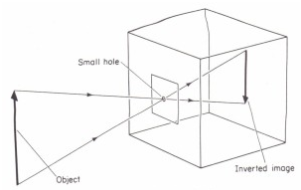
\includegraphics[width=8cm,height=8cm,keepaspectratio]{imagenes/pinhole.PNG}
\caption{Image formation by a pinhole camera }
\label{fig:pinhole}
\end{figure}
The advantage of a lens over a pinhole camera is the increased amount of light that is allowed to pass. A lens gathers an entire pencil of rays from each object pointed instead of a single ray. A lens placed in front of an object gathers a pencil of rays from each point's bundles of rays and brings these rays to focus at a point in a plane o the other side of the lens, called the image plane\cite{elements_photogrammetry}.
\begin{figure}[H]
\centering
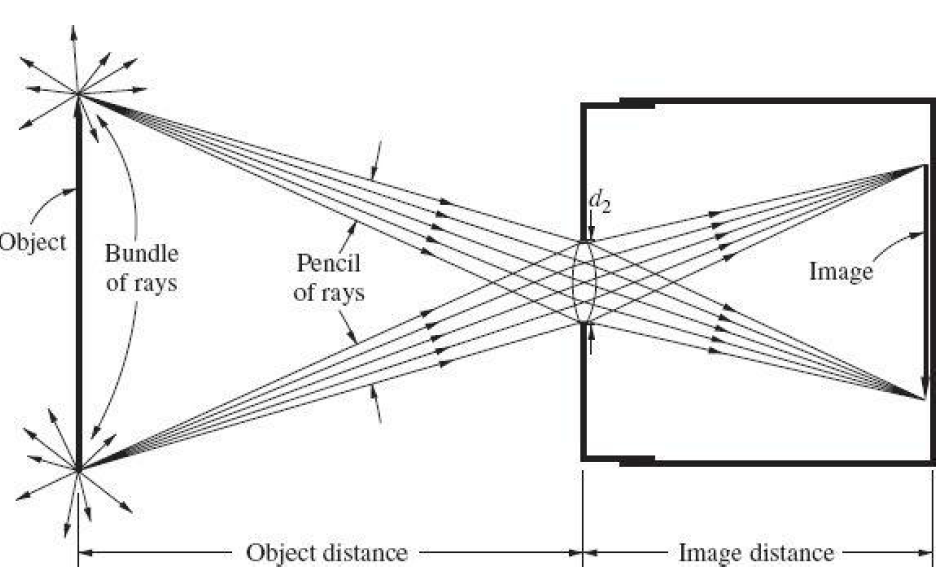
\includegraphics[width=8cm,height=8cm,keepaspectratio]{imagenes/lens.PNG}
\caption{pencils of light and image formation in a single-lens camera}
\label{fig:lens}
\end{figure}
The \textit{optical axis} of a lens is defined as the line joining the center of curvature of the spherical surface of the lens (point $O_{1}$ and $O_{2}$ in figure \ref{fig:optical_axis}). In this figure, $R_{1}$ and $R_{2}$ are the radii of the lens surface, and the optical axis is the line $O_{1}O_{2}$ light rays parallel to the optical axis as they enter the lens come to focus at \textit{F}, the \textit{focal point} of the lens. The distance from the focal point to the center of the lens is \textit{f}, the \textit{focal length}. A plane perpendicular to the optical axis passing through the focal point is called the \textit{plane of infinite focus} or simply \textit{focal plane}\cite{elements_photogrammetry}.
\begin{figure}[H]
\centering
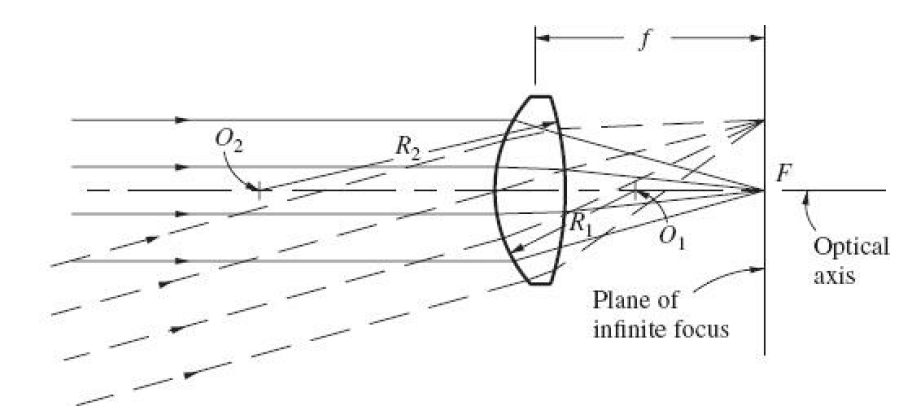
\includegraphics[width=9cm,height=9cm,keepaspectratio]{imagenes/optical_axis.PNG}
\caption{optical axis,focal length,and plane of infinite focus}
\label{fig:optical_axis}
\end{figure}
A pencil of incident light rays coming from an object locate an infinite distance away from the lens will be parallel, and the image will come to focus in the plane of infinite focus. For objects located some finite distance from the lens, the \textit{image distance} (distance from the lens center to the image plane) is greater than the focal length. the equation \ref{lens_formula} , called \textit{lens formula} expresses the relationship of object distance  \textit{o} and image distance \textit{i} to the focal length \textit{f} of a converging lens \cite{elements_photogrammetry}.:
\begin{equation}
\frac{1}{o}+\frac{1}{i}=\frac{1}{f}
\label{lens_formula}
\end{equation}
The \textit{depth of field} of a lens is the range in object distance that can be accommodated by the lens without introducing significant image deterioration. For a given lens, Increasing the depth of field can be obtained by reducing the size of the lens opening (\textit{aperture}). This phenomenon limits the usable area of the lens to the central portion, depth of field is extremely critical. The shorter the focal length of a lens, the greater its depth of field, and vice versa.\cite{elements_photogrammetry}
\subsubsection{Illuminance}
Illuminance of any photographic exposure is the brightness or amount of light received per unit of area on the image plane surface during exposure.
Illuminance is proportional to the amount of light passing through the lens opening during exposure, and this is proportional to the area of the opening. since the area of the lens opening is $\frac{\pi d^2}{4}$, illuminance is proportional to the variable $d^2$.\cite{elements_photogrammetry}

Image distance \textit{i} is another factor which affects illuminance. illuminance adheres to the inverse square law, which means that the amount of illuminance is inversely proportional to square distance from the aperture. According to the law, at the center of the photograph, illuminance is proportional to $\frac{1}{i^2}$ Normally in photography, object distances are sufficiently long that the term $\frac{1}{o}$ in equation \ref{lens_formula} is nearly zero.In which case \textit{i} is equal to \textit{f}. Thus the center of a photograph is proportional to $\frac{1}{f^2}$, and the two quantities may be combined so that illuminance is proportional to $\frac{d^2}{f^2}$. the square root of this term is called the \textit{brightness factor}\cite{elements_photogrammetry}
\begin{equation}
\sqrt[]{\frac{d^2}{f^2}}=\frac{d}{f}
\label{brightness}
\end{equation}
The inverse of equation \ref{brightness} is also an inverse expression of illuminance and is called \textit{f}-stop. In equation form, According to equation \ref{fstop},\textit{f}-stop is the ratio of focal length to the diameter of the lens opening, or \textit{aperture}. As the aperture increases, \textit{f}-stop numbers decreases and illuminance increases, thus requiring less exposure time.\cite{elements_photogrammetry}

Because the correlation between \textit{f}-stophttps://www.overleaf.com/18328668czpfwmrbbsvd and shutter speed, \textit{f}-stop is the term used for expressing \textit{lens speed} or the " light-gathering" power of a lens.Illuminance produced by a particular lens is computed using equation \ref{fstop}, weather the lens has a very small diameter with short focal length or a very large diameter with a long focal length.\cite{elements_photogrammetry}
\begin{equation}
f-stop=\frac{f}{d}
\label{fstop}
\end{equation}
\subsubsection{Relationship of aperture and Shutter speed}
Total exposure of photographic films is the product of illuminance and time of exposure.
Illuminance is regulated by varying \textit{f}-stop setting on the camera, while the time of exposure can by varying the shutter speed. Variation in the \textit{f}-stop setting is variation in the diameter of the aperture, which can be controlled by a diaphragm, changing the diameter of the opening of the lens and thus regulating the amount of light that is allowed to pass through the lens.\cite{elements_photogrammetry}.

With a lens camera, as the diameter of the aperture increases, enabling faster exposures, the depth of field becomes less and less distorted become more severe. To photograph a scene with great variation in object distances and yet retain the sharp focus of all images, a large depth of field is required. In this case, to maximize depth of field, the picture would be taken at a slow shutter speed and large \textit{f}-stop setting, corresponding to a small diameter lens opening. On the other hand, in photographing fast moving objects or in making exposures from a moving vehicle such an airplane, a fast shutter is essential, to reduce image motion. In this situation, a small \textit{f}-stop setting corresponding to a large diameter lens opening would be necessary for sufficient exposure.\cite{Planning_airborne}
\subsubsection{CCD,CMOS sensors and shutter types}
Two image sensor types widely used in cameras are Charge Coupled Devices (CCD) and Complementary Metal Oxide Semiconductors (CMOS) there are many similarities between the two technologies, but one major distinction is the way each sensor reads the signals accumulated at a given pixel. There is a difference in the readout modes, impact exposure timing, illumination, and triggering of cameras.

CCD sensor usually uses in a Global Shutter mode. In Global Shutter mode, every pixel is exposed simultaneously at the same instant in time. This situation is particularly beneficial when the image is changing from frame to frame. The CCD, however, has an inherent disadvantage when it comes to frame rate. When the exposure is complete, the cameras CCD transfers the signal from each pixel to a single Analog to Digital Converter

A CMOS chip eliminates this bottleneck by using an A/D for every column of pixels, which can number in the thousands. The total number of pixels digitized by anyone converter is significantly reduced, enabling shorter readout times and consequently faster frame rates. While there are many parallel A/D’s sharing the workload, the entire sensor array must still be converted one row at a time. This situation results in a small time delay between each row’s readout. 

Rather than waiting for an entire frame to complete readout, to further maximize frame rates, each row is typically able to begin the next frame’s exposure once completing the previous frame’s readout. While fast, the time delay between each row’s readout then translates to a delay between each row’s beginning of the exposure, making them no longer simultaneous. The result is that each row in a frame is exposed for the same amount of time but begin exposing at a different point in time, allowing overlapping exposures for two frames. The ultimate frame rate is determined by how quickly the rolling readout process can be completed. This Rolling Shutter mode is illustrated in Figure \ref{fig:Rolling} \cite{Shutter}

\begin{figure}[H]
\centering
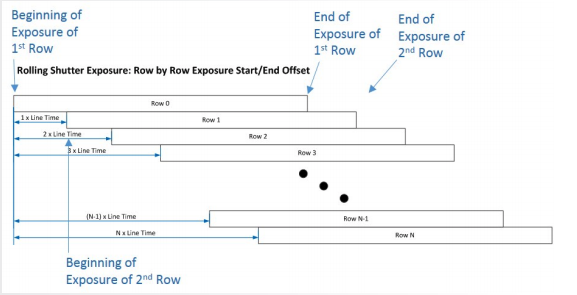
\includegraphics[width=10cm,height=8cm,keepaspectratio]{imagenes/Rolling.png}
\caption{Diagram demonstrating
the time delay between each row
of pixels in a rolling shutter readout
mode with a CMOS camera}
\label{fig:Rolling}
\end{figure}

\subsection{Photogrammetry}
Photogrammetry has been defined by the American Society for Photogrammetry and Remote Sensing as the art, science, and technology of obtaining reliable information about physical objects and the environment through processes of recording, measuring and interpreting photographic images and patterns of recorded electromagnetic energy or other phenomena. \cite{ASPRS}

Included within the definition of photogrammetry are two distinct areas: 1 metric photogrammetry and 2 interpretative photogrammetry. Metric photogrammetry consists of making precise measurements from photos or other information sources to determine, in general, the relative location of points. Enabling finding distances, angles, areas, volumes, elevations, sizes, and shapes of objects. The most common applications of metric photogrammetry are the preparation of orthophotos from digital imagery.

Interpretative photogrammetry deal principally in recognizing and identifying objects and judging their significance through careful and systematic analysis. It is included in the branches of image interpretation and remote sensing. Image interpretation and remote sensing include not only the analysis of photography but also the use of data gathered from a wide variety of sensing instruments, including multispectral cameras, infrared sensors, thermal scanners, and side looking airborne radar.\cite{elements_photogrammetry}
\subsubsection{types of photogrammetry}
Two fundamentals classification of photography used in the science of photogrammetry are terrestrial and aerial. 
\begin{itemize}
\item Terrestrial: photographs are taken with ground-based cameras the position and orientation of which might be measured directly at the time of exposure. A great variety of cameras are used for taking terrestrial photogrammetry, digital cameras have become the standard sensors for image acquisition 
\item Aerial: photography is commonly classified as either vertical or oblique. Vertical photos are taken with the camera axis directed as nearly as vertical as possible. If the camera axis were perfectly vertical when an exposure was made, the photographic plane would be parallel to the datum plane and the resulting photograph would be termed truly vertical. When the camera axis is unintentionally tilted slightly from vertical, the resulting photograph is called tilted photograph.\cite{elements_photogrammetry}
\end{itemize}
\subsection{Euler Angels}
According to Euler's rotation theorem, any rotation may be described using three angles. If  the rotation are written in terms of rotation matrices $R_{z}(\alpha),R_{y}(\beta),R_{y}(\gamma)$. Then a general rotation A can be written as:
\begin{equation}
A = R_{z}(\alpha)\cdot R_{y}(\beta)\cdot R_{y}(\gamma)
\end{equation}
The three angles giving the three rotation matrices are called Euler angles. There area several conventions for Euler angles, depending on the axes about witch the rotation are carried out. In aviation rotation is executed in a Z-Y-X order.\cite{Euler}.
\begin{figure}[H]
\centering
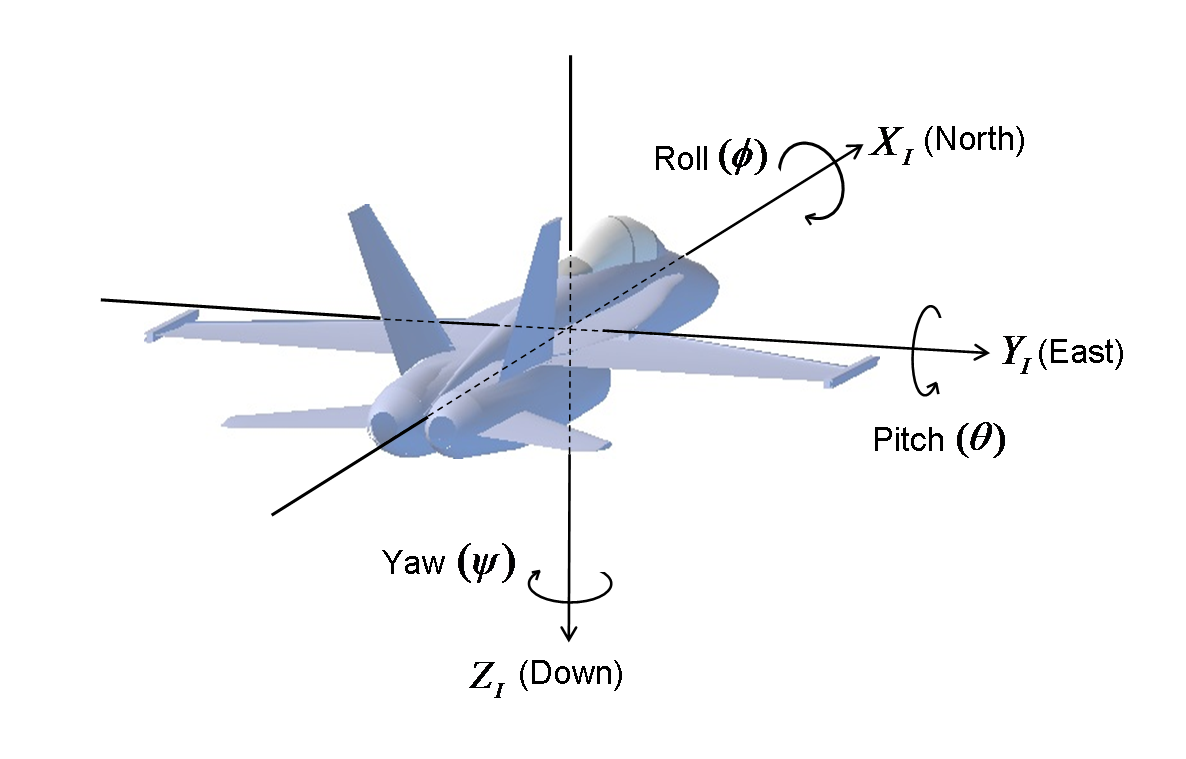
\includegraphics[width=10cm,height=10cm,keepaspectratio]{imagenes/Euler_Angles.png}
\caption{The Inertial Frame for a plane}
\label{fig:Euler}
\end{figure}
\subsubsection{Yaw}
Yaw is a counterclockwise rotation of $\alpha$ about the z-axis. the rotation matrix is given by.
\begin{equation}R_{z}(\alpha) =
\begin{bmatrix}cos(\alpha) & -sin(\alpha) & 0 \\sin(\alpha) & cos(\alpha)& 0\\0 &0&1 \end{bmatrix}
\end{equation}
note that the upper left entries of $R_{z}(\alpha)$ form a 2D rotation applied to the x and y coordinate, where areas the z coordinates remains constant.\cite{Euler_angles}
\subsubsection{Pitch}
A pitch is a counterclockwise rotation of $\beta$ about the y-axis. The rotation matrix is given by.
\begin{equation}R_{y}(\beta) =
\begin{bmatrix}cos(\beta) & 0 & sin(\beta) \\0 & 1& 0\\-sin(\beta) &0&cos(\beta) \end{bmatrix}
\end{equation}
\subsubsection{Roll}
A roll is a counterclockwise rotation of $\gamma$ about the x-axis. The rotation matrix is given by.
\begin{equation}R_{z}(\gamma) =
\begin{bmatrix}1 & 0 &0 \\0 &cos(\gamma))& -sin(\gamma) \\0 &sin(\gamma)&cos(\gamma) \end{bmatrix}
\end{equation}
Computing a rotation A in ZYX using the Euler's angles will result in:
\begin{equation}
A = \begin{bmatrix}cos(\alpha) & -sin(\alpha) & 0 \\sin(\alpha) & cos(\alpha)& 0\\0 &0&1 \end{bmatrix}
\cdot \begin{bmatrix}1 & 0 &0 \\0 &cos(\gamma))& -sin(\gamma) \\0 &sin(\gamma)&cos(\gamma) \end{bmatrix}
\cdot \begin{bmatrix}1 & 0 &0 \\0 &cos(\gamma))& -sin(\gamma) \\0 &sin(\gamma)&cos(\gamma) \end{bmatrix}
\end{equation}
\begin{equation}
\begin{bmatrix}cos(\alpha)\cdot  cos(\beta)& cos(\alpha)\cdot sin(\beta)\cdot sin(\gamma)-sin(\alpha)\cdot cos(\gamma)& cos(\alpha)\cdot sin(\beta)\cdot cos(\gamma)+sin(\alpha)\cdot sin(\gamma) \\ sin(\alpha)\cdot cos(\beta)& cos(\alpha)\cdot sin(\beta)\cdot sin(\gamma)+cos(\alpha)\cdot cos(\gamma)&sin(\alpha)\cdot sin(\beta)\cdot cos(\gamma)- cos(\alpha)\cdot sin(\gamma)\\ -sin(\beta) & cos(\beta)\cdot sin(\gamma) & cos(\beta)\cdot cos(\gamma) \end{bmatrix}
\end{equation}
\subsection{Mission planning} For UAV, the autonomy is characterized by its level of
interaction with the operator: the more abstract the operator decisions are, the more autonomous the vehicle is. Mission planning and flight scheduling, computing an appropriate path for the vehicle in order to achieve the objectives of the mission, is one of the main challenges for UAV development in order to increase the autonomy level. Usually, mission planning is used to describe all these tasks\cite{4281723}

The first step in the design is to decide on the scales or its resolution and the required accuracy. Once those two requirements are known, the following processes follow:
\begin{enumerate}
\item Planning the aerial photography (developing the flight plan);
\item Planning the ground controls;
\item Selecting software, instruments and procedures necessary to produce the final products
\end{enumerate}
For the flight plan, the planner needs to know the following information, some of which are computed.\cite{Design_plann}
\begin{itemize}
\item Focal length of the camera lens.
\item Flying height.
\item Size of the CCD.
\item Size of CCD Array (how many pixels).
\item Size and shape of the area to be photographed.
\item The amount of end lap and side lap.
\item Ground speed of aircraft.
\end{itemize}
\subsubsection{End lap and front lap}
When covering an area by vertical aerial photography, the photographs are usually taken along a series of parallel passes, called \textit{flight strips}. As shown in figure \ref{fig:EndLap}, the photographs are normally exposed in such a way that the area covered by each successive photograph along with a flight strip duplicates or overlaps part of the ground of the previous photo. This action is lapping along the flight strip is called \textit{end lap}, and the area coverage common to an adjacent pair of photographs in a flight strip is called the \textit{stereoscopic overlap area}. the overlapping pair of photo is called \textit{stereopair}\cite{elements_photogrammetry}.

\begin{figure}[H]
\centering
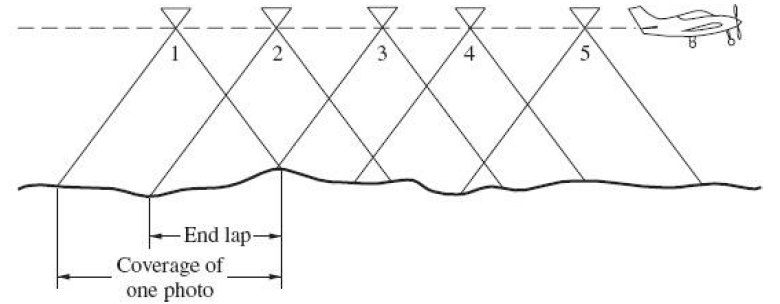
\includegraphics[width=10cm,height=10cm,keepaspectratio]{imagenes/EndLap.PNG}
\caption{End lap of photographs in a flight strip}
\label{fig:EndLap}
\end{figure}

Adjacent flight strips area photograph so that there is also a lateral overlapping of ground coverage between strips. This condition shown in figure \ref{fig:SideLap}, is called \textit{side lap}\cite{elements_photogrammetry}.
\begin{figure}[H]
\centering
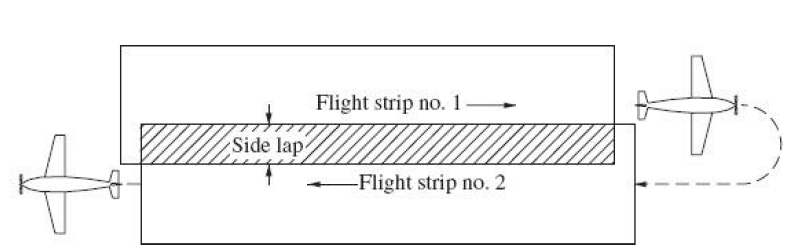
\includegraphics[width=10cm,height=10cm,keepaspectratio]{imagenes/sidelap.PNG}
\caption{Side lap of adjacent flight strips}
\label{fig:SideLap}
\end{figure}

\subsubsection{Ground Sampling Distance (GSD)}
The size of a pixel projected to the ground surface, as reported in linear units per pixel; for example, a USGS Digital Orthophoto Quarter Quad (DOQQ) has a 1-meter GSD because each pixel corresponds to 1 meter on the ground. GSD is what many people (and remote sensing product vendors) actually mean when they talk about the "spatial resolution" of an image; GSD is the correct term. When using the term in reference to an elevation model, GSD describes the actual or nominal spacing between ground elevation samples or measurements.\cite{Design_plann}.
\subsubsection{Flight height computation}
The flight height H that is need to obtain a given GSD can be computed and depends on the camera focal length, the camera sensor width  (mm), and the image width (pixels).\cite{GSDComputation}
\begin{figure}[H]
\centering
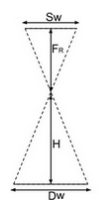
\includegraphics[width=4cm,height=4cm,keepaspectratio]{imagenes/GSD.PNG}
\caption{GSD variable definition}
\label{fig:GSD}
\end{figure}
\begin{table}[H]
\centering
\begin{tabular}{|c|c|}
\hline
\textbf{Variable} & \textbf{Definition}                                                                      \\ \hline
Sw                & Real sensor width (mm)                                                                   \\ \hline
FR                & Real Focal length (mm)                                                                   \\ \hline
H                 & Flight height (m)                                                                        \\ \hline
Dw                & Distance covered on the ground by one image (footprint width) (m) \\ \hline
\end{tabular}
\caption{GSD variable definition}
\end{table}
Using the fact that:
\begin{equation}
H/F_{R} = D_{w}/S_{w}
\end{equation}
The flight height H is given by:
\begin{equation}
H = (D_{W}\cdot F_{R})/S_{W}
\label{H}
\end{equation}
The distance covered on the ground by one image in the width direction (foot print width) is given by:
\begin{equation}
D_{w}=(imW*GSD)/100
\label{DW}
\end{equation}
\begin{table}[H]
\centering
\begin{tabular}{|c|c|}
\hline
\textbf{Variable} & \textbf{Definition}   \\ \hline
imW              & Image width (pixels)  \\ \hline
GSD               & Desire GSD (cm/pixel) \\ \hline
\end{tabular}
\caption{Height equation Variable definition}
\end{table}
Combining equations \ref{H} and \ref{DW}, the flight height is given by:
\begin{equation}
H[m]=(imW\cdot GSD \cdot F_{R})\cdot (S_{w}*100)
\end{equation}
Image shotting rate to achieve a given overlap depends on the speed of the UAS, the GSD and the pixel resolution of the camera.
\begin{table}[H]
\centering
\begin{tabular}{|c|c|}
\hline
Variable & Definition                                                                  \\ \hline
D        & Distance covered on the ground by one image in the flight direction {[}m{]} \\ \hline
Overlap  & percentage of desire frontal overlap between two images.                    \\ \hline
X        & Distance between two images in the flight direction. {[}m{]}                \\ \hline
V        & flight speed {[}m/s{]}                                                      \\ \hline
t        & elapsed time between two images (image rate) {[}s{]}                        \\ \hline
imH      & Image height {[}pixel{]}                                                    \\ \hline
\end{tabular}
\caption{Time equation variable definition}
\end{table}
\begin{figure}[H]
\centering
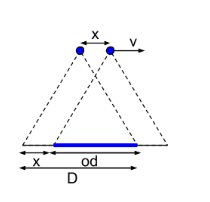
\includegraphics[width=6cm,height=6cm,keepaspectratio]{imagenes/velocity.PNG}
\caption{Velocity computing variables}
\label{fig:velocity}
\end{figure}
form figure \ref{fig:velocity}, we obtain the following equations:
\begin{equation}
od =overlap\cdot D
\label{od}
\end{equation}
\begin{equation}
x=D\cdot od
\label{x}
\end{equation}
\begin{equation}
t = x/v
\label{t}
\end{equation}
\begin{equation}
D=D_{h}=(imH\cdot GSD)/100
\label{D}
\end{equation}
Combining equations: \ref{od} and \ref{D} into equation \ref{x}:
\begin{equation}
x = D_{h}-overlap\cdot D_{h}
\end{equation}
\begin{equation}
x= D_{h\cdot (1-overlap)}
\end{equation}
\begin{equation}
x = ((imH\cdot GSD)/100)\cdot (1-overlap)
\label{X_large}
\end{equation}
Combing the equations \ref{t} and \ref{X_large}:
\begin{equation}
t=x/v=\frac{((imH\cdot GSD)/100)\cdot (1-overlap)}{v}
\end{equation}
\subsubsection{Flight path design}
For a rectangularly shaped project, always use the smallest dimension of the project area to layout your flight lines. This way it results in fewer flight lines and then less turns between flight lines. In Figure \ref{fig:line_orientaion}, the red lines with arrowheads represent flight lines or strips, while the black dash lines represent the project boundary.
\begin{figure}[H]
\centering
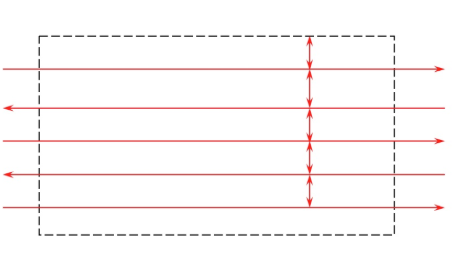
\includegraphics[width=10cm,height=10cm,keepaspectratio]{imagenes/flight_path.PNG}
\caption{Correct flight lines orientation}
\label{fig:line_orientaion}
\end{figure}
If you have a digital camera with a rectangular shape CCD array, always choose the largest dimension of the CCD array of the camera to be perpendicular to the flight direction. In Figure \ref{fig:camera_orientaion}, the blue rectangles represent images as taken by a camera with rectangular CCD array. The wider dimension of the array is always configured to be perpendicular to the flight direction\cite{GCP}
\begin{figure}[H]
\centering
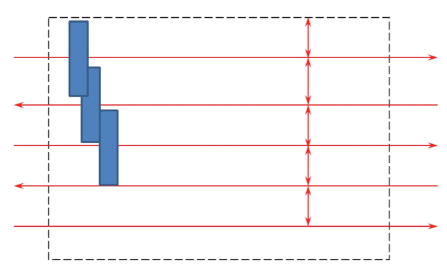
\includegraphics[width=10cm,height=10cm,keepaspectratio]{imagenes/flight_path_oritentation.PNG}
\caption{Correct camera orientation}
\label{fig:camera_orientaion}
\end{figure}
\begin{table}[H]
\centering
\begin{tabular}{|c|c|}
\hline
\textbf{Variable} & \textbf{Definition}                           \\ \hline
SP                & Line spacing or distance between flight lines \\ \hline
D                 & Image coverage                                \\ \hline
SL                & Amount of side lap                            \\ \hline
NFL               & Number of flight lines                        \\ \hline
\end{tabular}
\label{Flight line amount equation variable definition}
\end{table}
To procedure to compute the number of flight lines is shown in the following procedure.
\begin{enumerate}
\item Compute the coverage on the ground of one image using equation \ref{D}
\item Compute the flight lines spacing as follows:
\begin{equation}
SP = D\cdot \frac{(100-SL)}{100}
\end{equation}
\item Number of flight lines (NFL) is computed as follow:
\begin{equation}
NFL=\frac{width}{SP}+1
\end{equation}
\end{enumerate}
\begin{figure}[H]
\centering
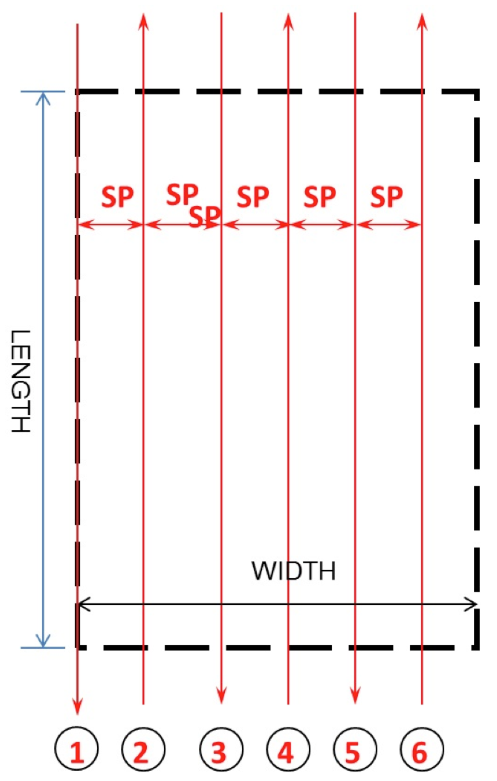
\includegraphics[width=10cm,height=10cm,keepaspectratio]{imagenes/flight_lines.PNG}
\caption {Flight line layouts}
\label{fig:flight_lines}
\end{figure}
\subsubsection{Geo-referencing images}
GPS loggers are very light devices (easily placed on a UAS) that can collect position information for the images. They register latitude, longitude and altitude values for each camera position while shooting. These values are saved to a file that can be imported into image processing software.\cite{GSDComputation}
\subsubsection{Ground control point GSP}
A ground control, is a target in the project area with known coordinates (X,Y,Z). Accurate, well placed ground controls are essential elements for any photogrammetric project utilizing aerial triangulation.\cite{Design_plann}

there are two standards types of ground control points, those are:
\begin{itemize}
\item Photo Identifiable (Photo ID): This could be any feature on the ground such as a manhole, parking stripe, etc. This type of control does not need to be surveyed before the UAS flies the project as it can be surveyed later on.\cite{Design_plann}
\item Pre-marked (Panels): This type is generated by marking or painting certain figures or symbols on the ground before the UAS flies the project \cite{Design_plann}
\end{itemize}
Ground control requirements vary from one project to another depending on the project specifications and its geographic extent. Projects with high geometrical accuracy requirements require more ground controls. Figure \ref{fig:GCP_sin} illustrates a typical distribution of ground controls in a rectangularly shaped project when the aircraft does not carry on board a GPS antenna, resulting in a non-GPS supported aerial triangulation, or what is usually called “conventional aerial triangulation.”\cite{GCP}
\begin{figure}[H]
\centering
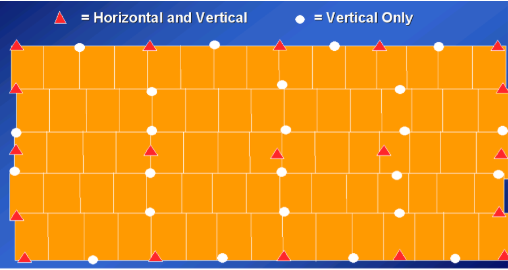
\includegraphics[width=6cm,height=6cm,keepaspectratio]{imagenes/GCP_sin.PNG}
\caption{ Ground control distribution in non-GPS supported aerial triangulation }
\label{fig:GCP_sin}
\end{figure}
